\documentclass{beamer}

\usepackage[magyar]{babel}

\author{Sándor Tibor}
\date{\today}
\title{Napelemes Adatok Feldolgozása}
\institute{MOGI tanszék}

\usepackage[outputdir=build]{minted}

\usetheme{Frankfurt}

\usepackage{graphicx}

\begin{document}

\frame{\titlepage}

\begin{frame}
  \frametitle{Motiváció}

  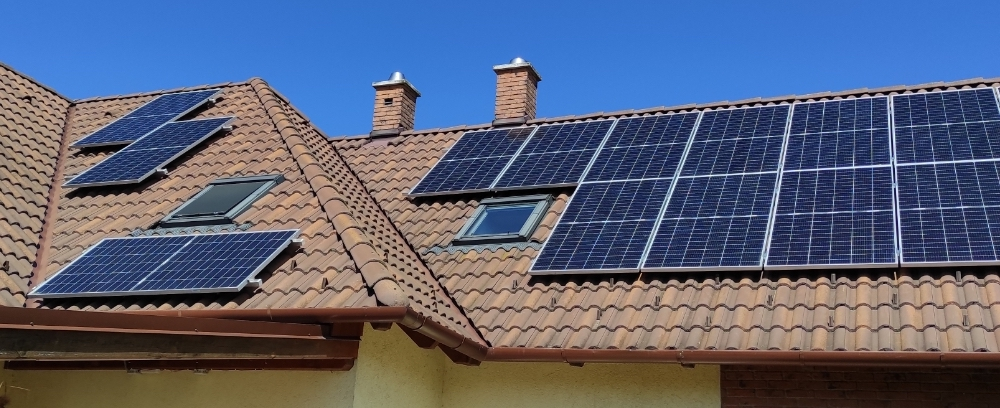
\includegraphics[width=\textwidth]{static/home.jpg}
\end{frame}

\begin{frame}[fragile]
  \frametitle{Express API}
  \framesubtitle

  
\includegraphics[height=1.25cm]{static/express-logo.png}\hfill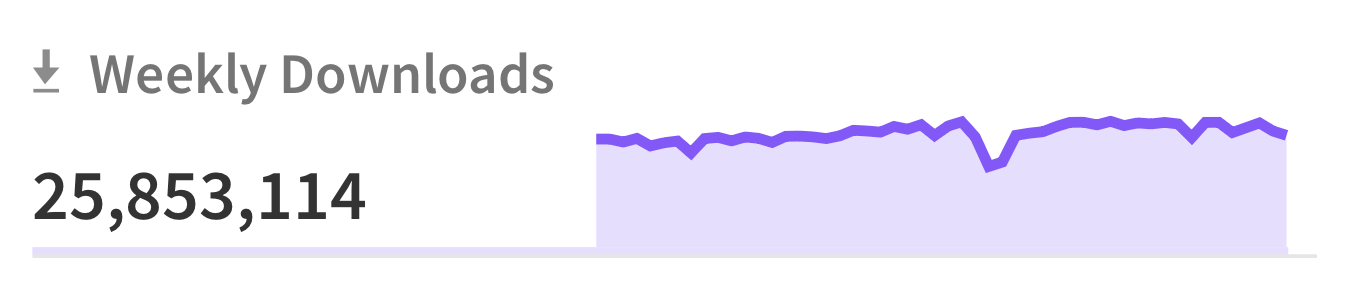
\includegraphics[height=1.25cm]{static/express-dowloads.png}

  \vfill

  \begin{minted}[fontsize=\small]{typescript}
const express = require('express');
const app = express();

app.get('/', function (req, res) {
  res.send('Hello World')
});

app.listen(process.env.PORT || 3000);
  \end{minted}

  \vfill
\end{frame}

\begin{frame}[fragile]
  \frametitle{Adatok}
  \framesubtitle{Általános Adatok}

  \begin{minipage}{.35\textwidth}
    \begin{minted}[fontsize=\small]{json}
{
  "dates": [ 
    "2023-05-24"
  ],
  "count": {
    "inverter": 8,
    "panel": 4
  }
}
    \end{minted}
  \end{minipage}\begin{minipage}{.45\textwidth}
    \begin{minted}[fontsize=\small]{typescript}
type About = {
  dates: Array<DateString>;
  count: {
    inverter: number;
    panel: number;
  };
};
    \end{minted}
  \end{minipage}\begin{minipage}{.15\textwidth}
    \flushright
    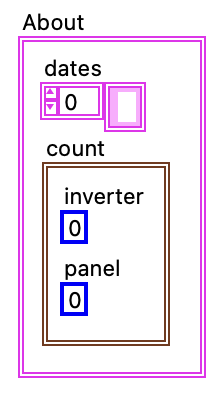
\includegraphics[height=4cm]{static/lv-about.png}
  \end{minipage}

\end{frame}

\begin{frame}[fragile]
  \frametitle{Adatok}
  \framesubtitle{Panel Adatok}

  \begin{minipage}[fontsize=\small]{.25\textwidth}
    \begin{minted}{json}
[
  3011,
  3047,
  // ...
  2595
]
    \end{minted}
  \end{minipage}\begin{minipage}{.5\textwidth}
    \begin{minted}[fontsize=\small]{typescript}
type Panel = Array<number>;
    \end{minted}
  \end{minipage}\begin{minipage}{.25\textwidth}
    \flushright
    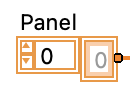
\includegraphics[height=2cm]{static/lv-panel.png}
  \end{minipage}
\end{frame}

\begin{frame}[fragile]
  \frametitle{Adatok}
  \framesubtitle{Részletes Adatok}

  \begin{minipage}{.3\textwidth}
    \begin{minted}[fontsize=\small]{json}
{
  "power": [
    0,
    // ...
  ],
  "sum": [
    0,
    // ...
  ],
  "hour": [
    "00:00",
    // ...
  ]
}
    \end{minted}
  \end{minipage}\begin{minipage}{.45\textwidth}
    \begin{minted}[fontsize=\small]{typescript}
type Detailed = {
  power: Array<number>;
  sum: Array<number>;
  hour: Array<string>;
}:
    \end{minted}
  \end{minipage}\begin{minipage}{.25\textwidth}
    \flushright
    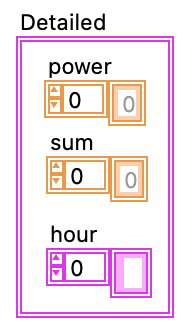
\includegraphics[height=6cm]{static/lv-detailed.png}
  \end{minipage}
\end{frame}

\begin{frame}
  \frametitle{Projekt választása}
  \framesubtitle{\;}

  \centering
  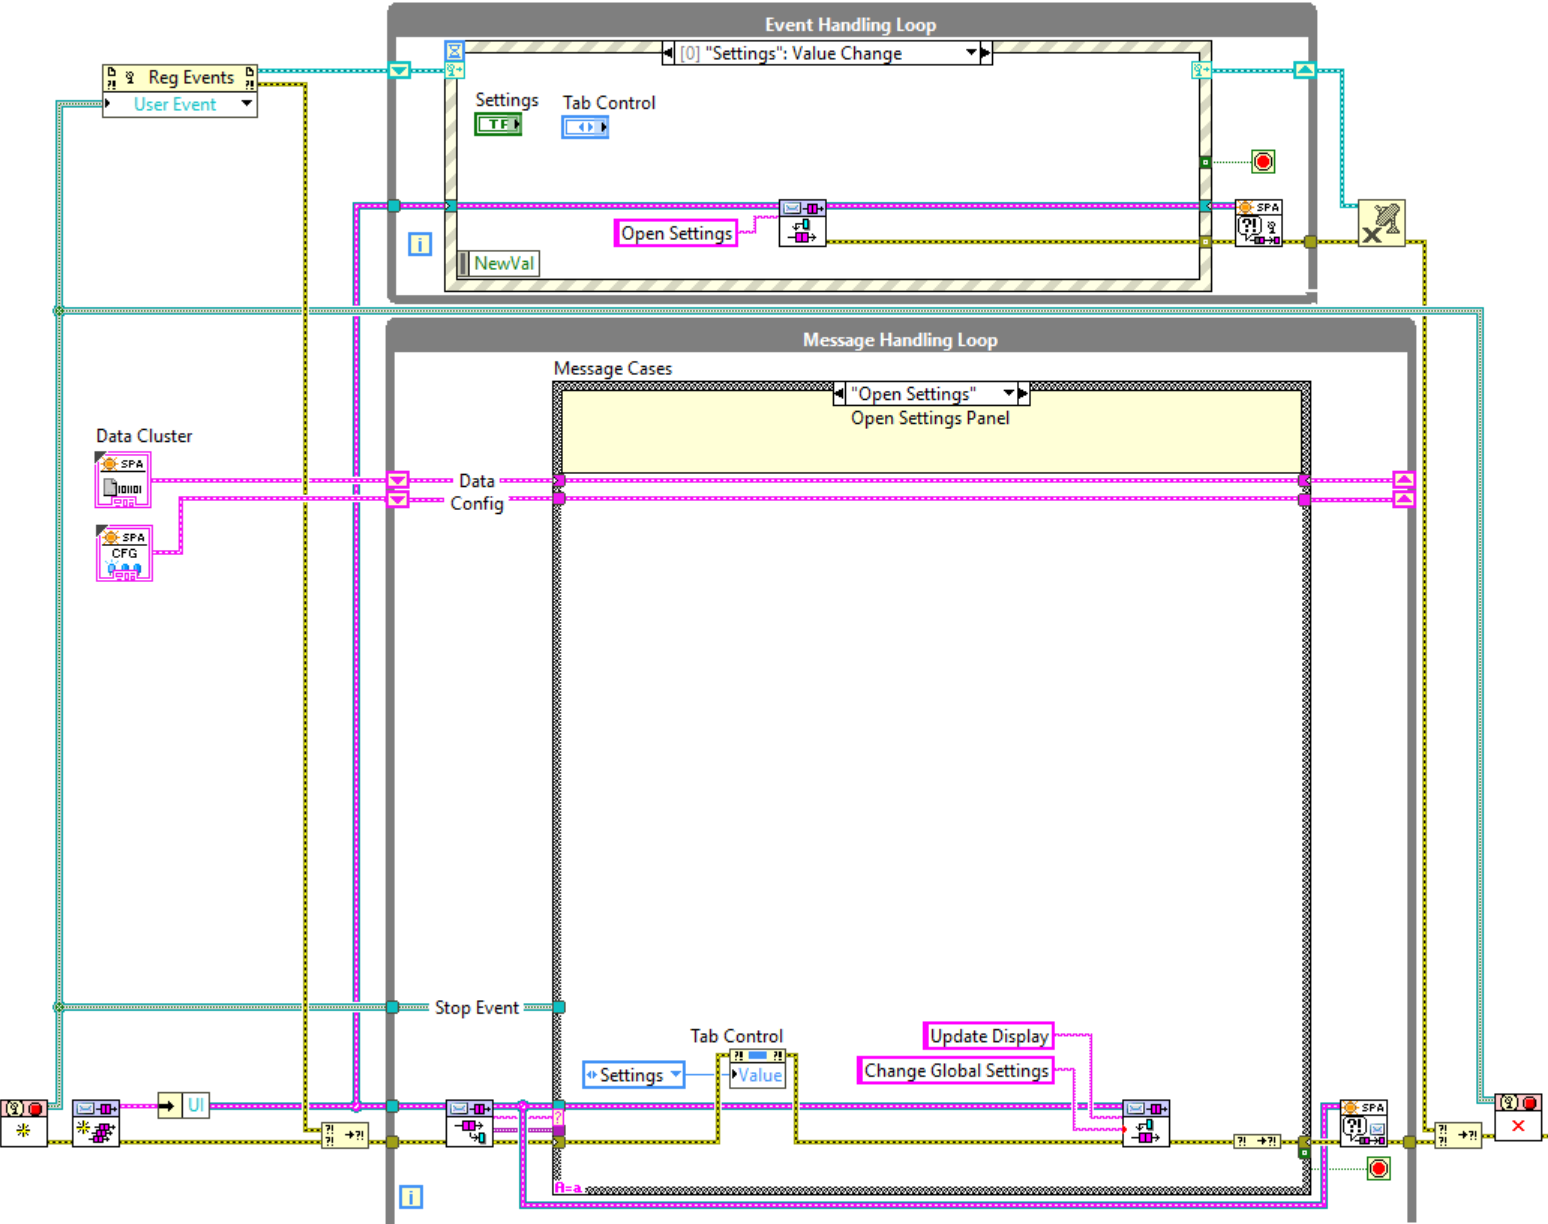
\includegraphics[height=.65\textwidth]{static/windows-bd.png}
\end{frame}

\begin{frame}
  \frametitle{Αdatok megjelenítése}
  \framesubtitle{Grafikonok}

  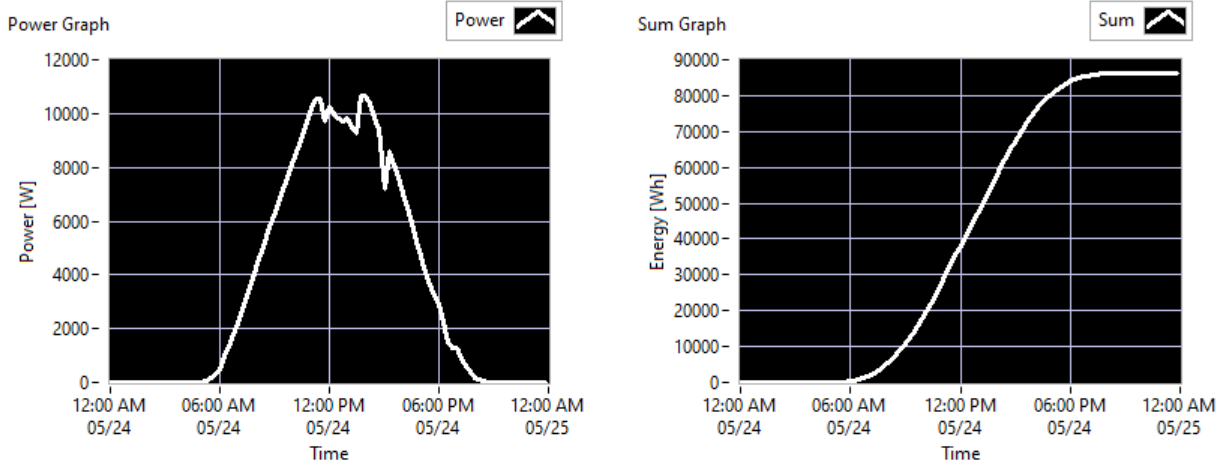
\includegraphics[width=\textwidth]{static/windows-graph.png}
\end{frame}

\begin{frame}
  \frametitle{Αdatok megjelenítése}
  \framesubtitle{Inverteres adatok}

  \centering
  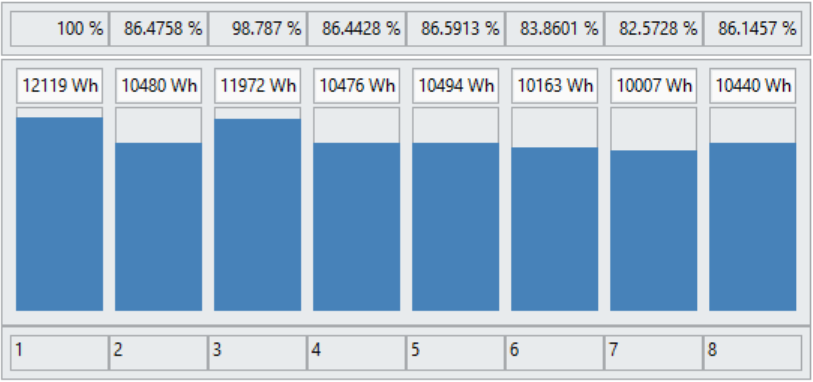
\includegraphics[width=\textwidth]{static/windows-inverter-energy.png}
\end{frame}

\begin{frame}
  \frametitle{Αdatok megjelenítése}
  \framesubtitle{Paneles adatok}

  \centering
  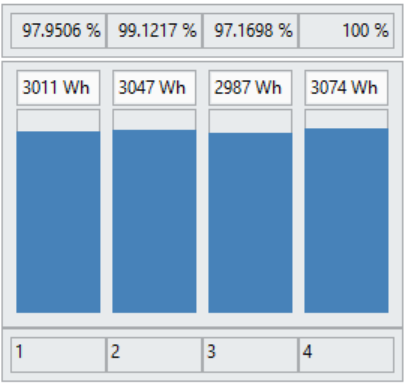
\includegraphics[width=.5\textwidth]{static/windows-panel-energy.png}
\end{frame}

\begin{frame}
  \frametitle{Αdatok megjelenítése}
  \framesubtitle{Kívánt adatok kiválasztása}

  \centering
  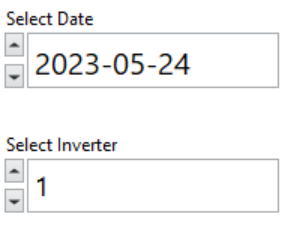
\includegraphics[width=.5\textwidth]{static/windows-ring.png}
\end{frame}

\begin{frame}
  \frametitle{Αdatok megjelenítése}
  \framesubtitle{A teljes front panel}

  \centering
  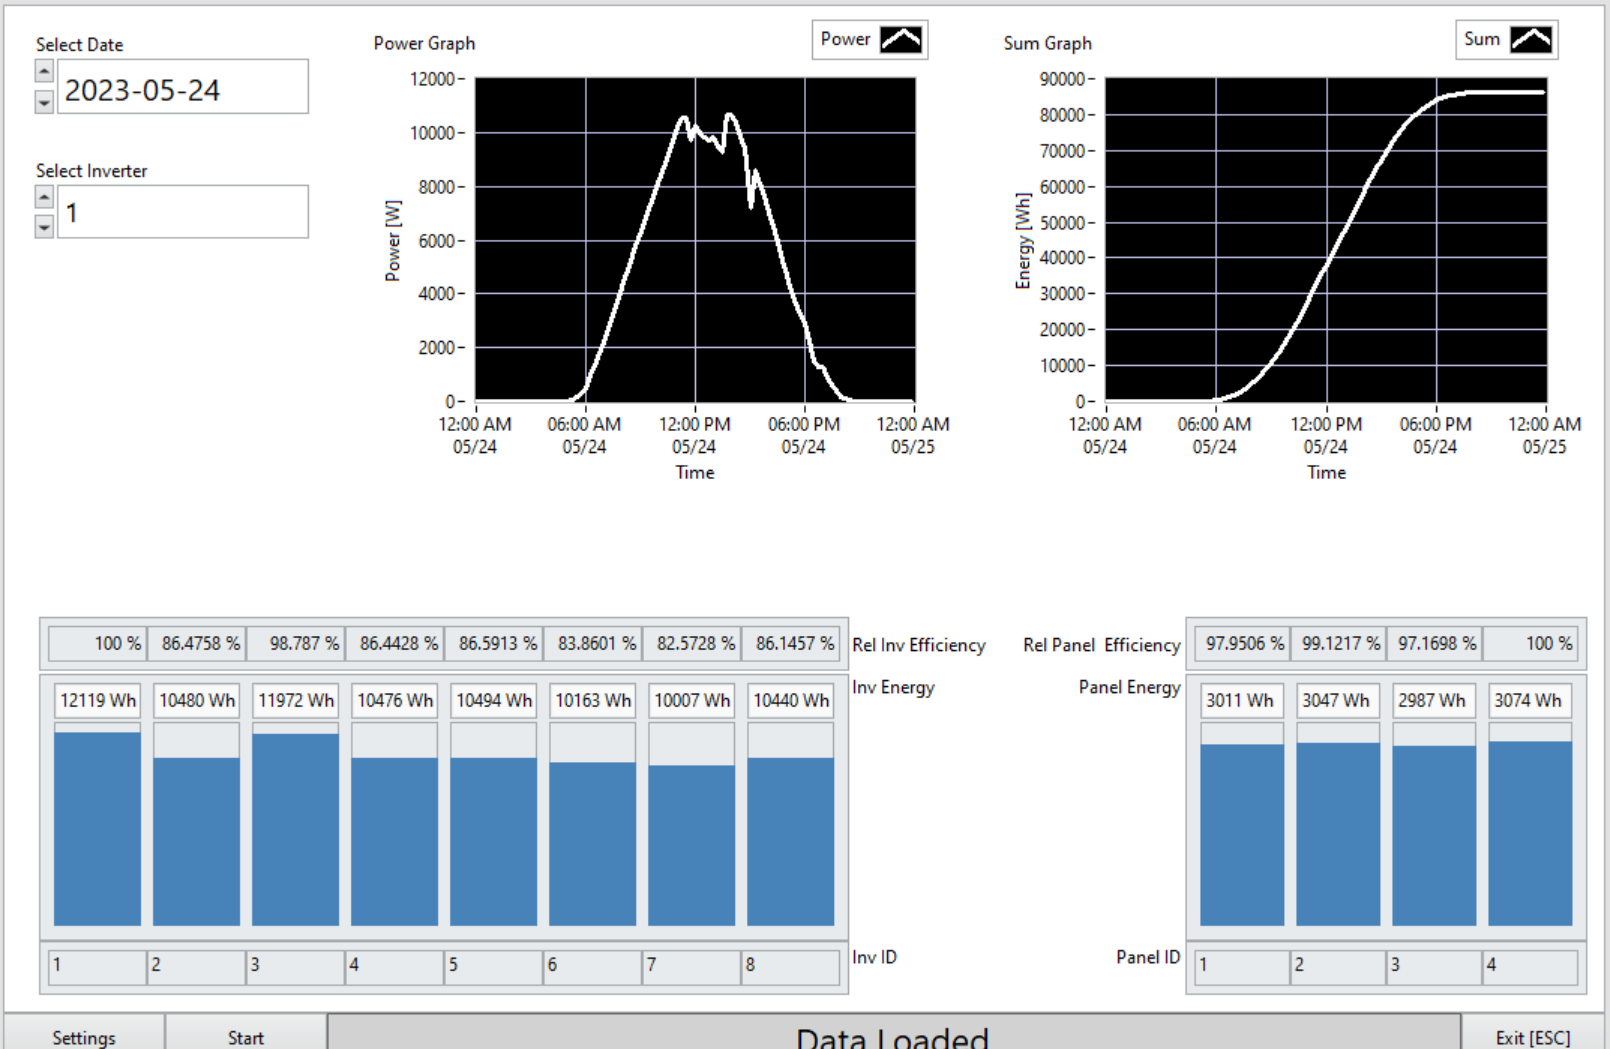
\includegraphics[height=.65\textwidth]{static/windows-fp.png}
\end{frame}

\begin{frame}
  \frametitle{\;}
  \framesubtitle{}

  \centering
  {
    \LARGE\bfseries
    Köszönöm szépen a figyelmet!
  }
\end{frame}

\end{document}
